\documentclass{article}
\usepackage{tikz}
\usetikzlibrary{matrix, positioning}

\begin{document}

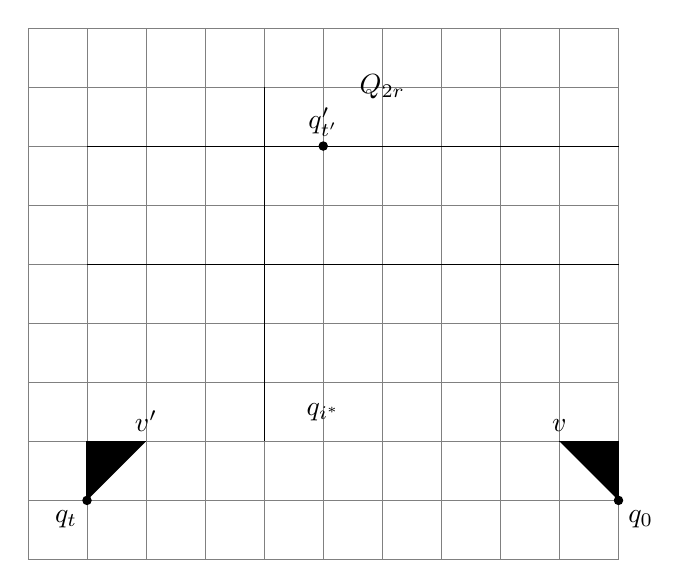
\begin{tikzpicture}[scale=0.75]
    \draw[help lines] (-1,-1) grid (9,8);
    
    % Drawing the main structure
    \draw (0,4) -- ++(9,0);
    \draw (0,6) -- ++(9,0);
    \draw (3,1) -- ++(0,6);
    
    % Highlighting specific cells
    \filldraw[black] (0,0) circle (2pt) node[below left] {$q_t$};
    \filldraw[black] (0,0) -- (0,1) -- (1,1) node[above] {$v'$};
    \filldraw[black] (9,0) circle (2pt) node[below right] {$q_0$};
    \filldraw[black] (9,0) -- (9,1) -- (8,1) node[above] {$v$};
    \filldraw[black] (4,6) circle (2pt) node[above] {$q_{t'}'$};
    
    % Labelling the area
    \node at (5,7) {$Q_{2r}$};
    \node at (4,1.5) {$q_{i^*}$};
\end{tikzpicture}

\captionof{figure}{Sketch for the construction of a short odd cycle containing \( v \), in the case \( d=2 \), when both \( v \) and its blue neighbour \( v' \) lie outside \( Q_{2r} \). The highlighted cells are used to construct paths from \( v \) and \( v' \) to \( q'_{t'} \), where an application of \cref{claim:paths} allows to close them into a cycle.}
\label{fig:construction_odd_cycle}

\end{document}